% Created by tikzDevice version 0.12.6 on 2026-01-28 16:24:46
% !TEX encoding = UTF-8 Unicode
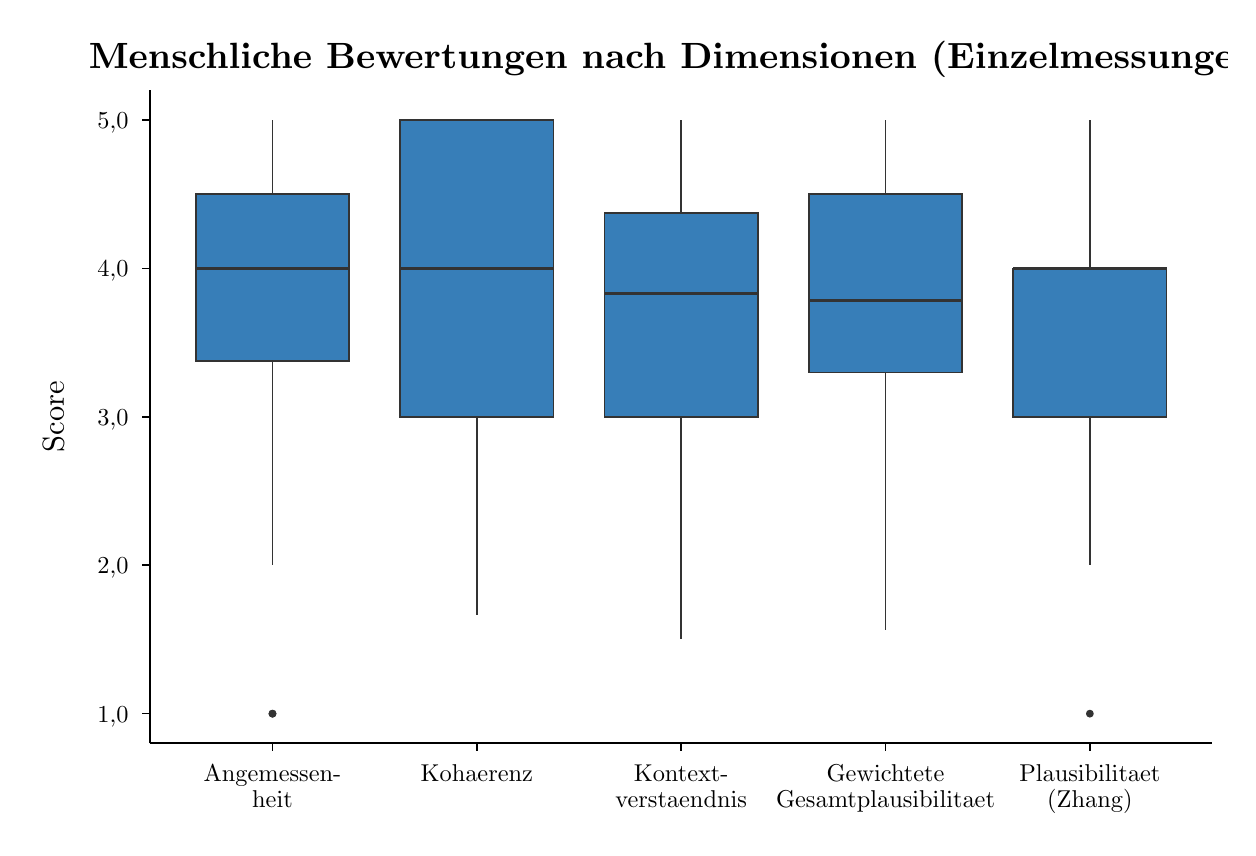
\begin{tikzpicture}[x=1pt,y=1pt]
\definecolor{fillColor}{RGB}{255,255,255}
\path[use as bounding box,fill=fillColor,fill opacity=0.00] (0,0) rectangle (433.62,289.08);
\begin{scope}
\path[clip] (  0.00,  0.00) rectangle (433.62,289.08);
\definecolor{fillColor}{RGB}{255,255,255}

\path[fill=fillColor] (  0.00,  0.00) rectangle (433.62,289.08);
\end{scope}
\begin{scope}
\path[clip] ( 44.16, 30.48) rectangle (428.12,266.40);
\definecolor{drawColor}{gray}{0.20}
\definecolor{fillColor}{gray}{0.20}

\path[draw=drawColor,line width= 0.4pt,line join=round,line cap=round,fill=fillColor] ( 88.46, 41.20) circle (  1.21);

\path[draw=drawColor,line width= 0.4pt,line join=round,line cap=round,fill=fillColor] ( 88.46, 41.20) circle (  1.21);

\path[draw=drawColor,line width= 0.6pt,line join=round] ( 88.46,228.87) -- ( 88.46,255.68);

\path[draw=drawColor,line width= 0.6pt,line join=round] ( 88.46,168.55) -- ( 88.46, 94.82);
\definecolor{fillColor}{RGB}{55,126,184}

\path[draw=drawColor,line width= 0.6pt,fill=fillColor] ( 60.77,228.87) --
	( 60.77,168.55) --
	(116.15,168.55) --
	(116.15,228.87) --
	( 60.77,228.87) --
	cycle;

\path[draw=drawColor,line width= 1.1pt] ( 60.77,202.06) -- (116.15,202.06);

\path[draw=drawColor,line width= 0.6pt,line join=round] (162.30,255.68) -- (162.30,255.68);

\path[draw=drawColor,line width= 0.6pt,line join=round] (162.30,148.44) -- (162.30, 76.95);

\path[draw=drawColor,line width= 0.6pt,fill=fillColor] (134.61,255.68) --
	(134.61,148.44) --
	(189.99,148.44) --
	(189.99,255.68) --
	(134.61,255.68) --
	cycle;

\path[draw=drawColor,line width= 1.1pt] (134.61,202.06) -- (189.99,202.06);

\path[draw=drawColor,line width= 0.6pt,line join=round] (236.14,222.17) -- (236.14,255.68);

\path[draw=drawColor,line width= 0.6pt,line join=round] (236.14,148.44) -- (236.14, 68.01);

\path[draw=drawColor,line width= 0.6pt,fill=fillColor] (208.45,222.17) --
	(208.45,148.44) --
	(263.83,148.44) --
	(263.83,222.17) --
	(208.45,222.17) --
	cycle;

\path[draw=drawColor,line width= 1.1pt] (208.45,193.12) -- (263.83,193.12);

\path[draw=drawColor,line width= 0.6pt,line join=round] (309.98,229.09) -- (309.98,255.68);

\path[draw=drawColor,line width= 0.6pt,line join=round] (309.98,164.53) -- (309.98, 71.58);

\path[draw=drawColor,line width= 0.6pt,fill=fillColor] (282.29,229.09) --
	(282.29,164.53) --
	(337.67,164.53) --
	(337.67,229.09) --
	(282.29,229.09) --
	cycle;

\path[draw=drawColor,line width= 1.1pt] (282.29,190.44) -- (337.67,190.44);
\definecolor{fillColor}{gray}{0.20}

\path[draw=drawColor,line width= 0.4pt,line join=round,line cap=round,fill=fillColor] (383.82, 41.20) circle (  1.21);

\path[draw=drawColor,line width= 0.6pt,line join=round] (383.82,202.06) -- (383.82,255.68);

\path[draw=drawColor,line width= 0.6pt,line join=round] (383.82,148.44) -- (383.82, 94.82);
\definecolor{fillColor}{RGB}{55,126,184}

\path[draw=drawColor,line width= 0.6pt,fill=fillColor] (356.13,202.06) --
	(356.13,148.44) --
	(411.51,148.44) --
	(411.51,202.06) --
	(356.13,202.06) --
	cycle;

\path[draw=drawColor,line width= 1.1pt] (356.13,202.06) -- (411.51,202.06);
\end{scope}
\begin{scope}
\path[clip] (  0.00,  0.00) rectangle (433.62,289.08);
\definecolor{drawColor}{RGB}{0,0,0}

\path[draw=drawColor,line width= 0.6pt,line join=round] ( 44.16, 30.48) --
	( 44.16,266.40);
\end{scope}
\begin{scope}
\path[clip] (  0.00,  0.00) rectangle (433.62,289.08);
\definecolor{drawColor}{RGB}{0,0,0}

\node[text=drawColor,anchor=base east,inner sep=0pt, outer sep=0pt, scale=  0.88] at ( 36.46, 38.17) {1,0};

\node[text=drawColor,anchor=base east,inner sep=0pt, outer sep=0pt, scale=  0.88] at ( 36.46, 91.79) {2,0};

\node[text=drawColor,anchor=base east,inner sep=0pt, outer sep=0pt, scale=  0.88] at ( 36.46,145.41) {3,0};

\node[text=drawColor,anchor=base east,inner sep=0pt, outer sep=0pt, scale=  0.88] at ( 36.46,199.03) {4,0};

\node[text=drawColor,anchor=base east,inner sep=0pt, outer sep=0pt, scale=  0.88] at ( 36.46,252.65) {5,0};
\end{scope}
\begin{scope}
\path[clip] (  0.00,  0.00) rectangle (433.62,289.08);
\definecolor{drawColor}{RGB}{0,0,0}

\path[draw=drawColor,line width= 0.6pt,line join=round] ( 41.41, 41.20) --
	( 44.16, 41.20);

\path[draw=drawColor,line width= 0.6pt,line join=round] ( 41.41, 94.82) --
	( 44.16, 94.82);

\path[draw=drawColor,line width= 0.6pt,line join=round] ( 41.41,148.44) --
	( 44.16,148.44);

\path[draw=drawColor,line width= 0.6pt,line join=round] ( 41.41,202.06) --
	( 44.16,202.06);

\path[draw=drawColor,line width= 0.6pt,line join=round] ( 41.41,255.68) --
	( 44.16,255.68);
\end{scope}
\begin{scope}
\path[clip] (  0.00,  0.00) rectangle (433.62,289.08);
\definecolor{drawColor}{RGB}{0,0,0}

\path[draw=drawColor,line width= 0.6pt,line join=round] ( 44.16, 30.48) --
	(428.12, 30.48);
\end{scope}
\begin{scope}
\path[clip] (  0.00,  0.00) rectangle (433.62,289.08);
\definecolor{drawColor}{RGB}{0,0,0}

\path[draw=drawColor,line width= 0.6pt,line join=round] ( 88.46, 27.73) --
	( 88.46, 30.48);

\path[draw=drawColor,line width= 0.6pt,line join=round] (162.30, 27.73) --
	(162.30, 30.48);

\path[draw=drawColor,line width= 0.6pt,line join=round] (236.14, 27.73) --
	(236.14, 30.48);

\path[draw=drawColor,line width= 0.6pt,line join=round] (309.98, 27.73) --
	(309.98, 30.48);

\path[draw=drawColor,line width= 0.6pt,line join=round] (383.82, 27.73) --
	(383.82, 30.48);
\end{scope}
\begin{scope}
\path[clip] (  0.00,  0.00) rectangle (433.62,289.08);
\definecolor{drawColor}{RGB}{0,0,0}

\node[text=drawColor,anchor=base,inner sep=0pt, outer sep=0pt, scale=  0.88] at ( 88.46, 16.71) {Angemessen-};

\node[text=drawColor,anchor=base,inner sep=0pt, outer sep=0pt, scale=  0.88] at ( 88.46,  7.21) {heit};

\node[text=drawColor,anchor=base,inner sep=0pt, outer sep=0pt, scale=  0.88] at (162.30, 16.71) {Kohaerenz};

\node[text=drawColor,anchor=base,inner sep=0pt, outer sep=0pt, scale=  0.88] at (236.14, 16.71) {Kontext-};

\node[text=drawColor,anchor=base,inner sep=0pt, outer sep=0pt, scale=  0.88] at (236.14,  7.21) {verstaendnis};

\node[text=drawColor,anchor=base,inner sep=0pt, outer sep=0pt, scale=  0.88] at (309.98, 16.71) {Gewichtete};

\node[text=drawColor,anchor=base,inner sep=0pt, outer sep=0pt, scale=  0.88] at (309.98,  7.21) {Gesamtplausibilitaet};

\node[text=drawColor,anchor=base,inner sep=0pt, outer sep=0pt, scale=  0.88] at (383.82, 16.71) {Plausibilitaet};

\node[text=drawColor,anchor=base,inner sep=0pt, outer sep=0pt, scale=  0.88] at (383.82,  7.21) {(Zhang)};
\end{scope}
\begin{scope}
\path[clip] (  0.00,  0.00) rectangle (433.62,289.08);
\definecolor{drawColor}{RGB}{0,0,0}

\node[text=drawColor,rotate= 90.00,anchor=base,inner sep=0pt, outer sep=0pt, scale=  1.10] at ( 13.08,148.44) {Score};
\end{scope}
\begin{scope}
\path[clip] (  0.00,  0.00) rectangle (433.62,289.08);
\definecolor{drawColor}{RGB}{0,0,0}

\node[text=drawColor,anchor=base,inner sep=0pt, outer sep=0pt, scale=  1.32] at (236.14,274.47) {\bfseries Menschliche Bewertungen nach Dimensionen (Einzelmessungen)};
\end{scope}
\end{tikzpicture}
